%
%-----------------------------------
\section{Rate equations model}
\label{sec:rate-equations-model}
%-----------------------------------
%

A simple approach to introduce the essential aspects of atom-light interaction was proposed by Einstein in 1917. Although this theory does not take coherent effects into account, it is justified within the quantum mechanics framework in appropriate limits. Einstein assumed discrete energy levels for both atom and light. In this context, the electromagnetic radiation is composed of packets of energy $ \hbar \omega $ and momentum $ \hbar \omega / c $ known as photons, where $ \omega $ is the angular frequency, $ \hbar = h / 2\pi$ is the reduced Planck constant, and $ c $ is the speed of light. Einstein also postulated phenomenological rate equations to describe two-level atomic transitions due to the absorption and emission of photons. Let us consider a two-level transition where the energy difference between the upper and lower level is $ \hbar \omega_0 $, and an electromagnetic radiation with spectral energy density $ u(\omega) $. In Figure \ref{fig:optical-transitions}, we illustrated the three possible transitions involving absorption and emission of photons.

Let us consider a dilute atomic gas with number density $ n_1(t) $ of atoms in the lower level and number density $ n_2(t) $ of atoms in the upper level after a period of time $ t $. The Einstein rate equations express the time evolution of $ n_1 $ and $ n_2 $ so that
\begin{equation}
	\frac{d n_1}{dt} = - \frac{d n_2}{dt} = - B_{12} u(\omega_0) n_1 + B_{21} u(\omega_0) n_2 + A n_2,
	\label{eq:Einstein-rate-equations}
\end{equation}
where $ B_{12} u(\omega_0) $, $ B_{21} u(\omega_0) $, and $ A $ are phenomenological rates associated with the stimulated absorption, stimulated emission and spontaneous emission respectively. The rates associated with stimulated processes are proportional to the spectral density energy and therefore theses processes only happen in the presence of a light field. 

\begin{figure}[H]
	\caption{Optical two-level transitions}
	\begin{subfigure}[t]{0.32\textwidth}
		\centering
		\subcaption{\textbf{Stimulated absorption}}
		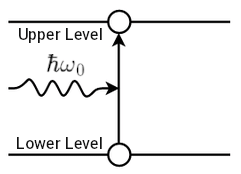
\includegraphics[width=0.8\textwidth]{USPSC-img/stimulated_absorption.png}
		\vspace{5pt}
		\legend{An atom in the lower level goes into the upper level absorbing a photon with energy $ \hbar \omega_0 $ from a light field with $ u(\omega_0) > 0 $.}
		\label{img:stimulated-absorption}
	\end{subfigure}
	\hfill
	\begin{subfigure}[t]{0.32\textwidth}
		\centering
		\subcaption{\textbf{Stimulated emission}}
		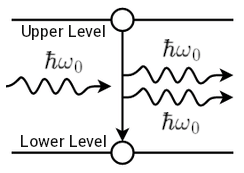
\includegraphics[width=0.8\textwidth]{USPSC-img/stimulated_emission.png}
		\vspace{5pt}
		\legend{An atom in the upper level decays into the lower level in the presence of a light field with $ u(\omega_0) > 0 $, emitting a photon with energy $\hbar \omega_0 $ similar to the photons in the light field.}
		\label{img:stimulated-emission}
	\end{subfigure}
	\hfill
	\begin{subfigure}[t]{0.32\textwidth}
		\centering
		\subcaption{\textbf{Spontaneous emission}}
		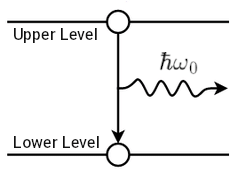
\includegraphics[width=0.8\textwidth]{USPSC-img/spontaneous_emission.png}
		\vspace{5pt}
		\legend{An atom in the upper level emits an isotropic photon with energy $ \hbar \omega_0 $ spontaneously, decaying into the lower level.}
		\label{img:spontaneous-emission}
	\end{subfigure}

	\legend{Source: Author}
	\vspace{-20pt}
	\label{fig:optical-transitions}
\end{figure}

%
%-----------------------------------
\subsection{Relation between the Einstein coefficients}
%-----------------------------------
%

A dilute atomic gas at temperature $ T $ in thermal equilibrium establishes a steady state in which $ n_1 $ and $ n_2 $ are constants of time ($ d_{t} n_1 = - d_{t} n_2 = 0 $). In this condition, from equation (\ref{eq:Einstein-rate-equations}), the spectral energy density is
\begin{equation}
	u({\omega_0}) = \frac{A}{(n_1 / n_2) B_{12} - B_{21}}.
	\label{eq:spectral-energy-thermal-equilibrium}
\end{equation}
Considering a fixed number of atoms $ n = n_1 + n_2 $, the system are represented by the canonical ensemble and then the ratio $ n_1 / n_2 $ is associated with the Boltzmann distribution so that
\begin{equation}
	\frac{n_1}{n_2} = \frac{g_1}{g_2} \exp\left\{-\frac{\hbar \omega_0}{k_B T}\right\},
	\label{eq:Boltzmann-distribution}
\end{equation}
where $ g_1 $ and $ g_2 $ are the degeneracies of the lower and upper level, respectively, and $ k_B $ is the Boltzmann constant. Einstein evaluated atoms in a region of black body radiation,  in which the spectral energy density of the light is consistent with the Planck distribution law given by
\begin{equation}
	u(\omega_0) = \frac{\hbar \omega_0^3}{\pi^2 c^3} \frac{1}{e^{\hbar \omega_0 / k_B T} - 1}.
	\label{eq:Planck-distribution}
\end{equation}
Comparing (\ref{eq:spectral-energy-thermal-equilibrium}), (\ref{eq:Boltzmann-distribution}), and (\ref{eq:Planck-distribution}), we obtain
\begin{equation} 
	B \equiv B_{21} = \frac{g_1}{g_2} B_{12}
	\label{eq:relation-B21-B12}
\end{equation}
and
\begin{equation} 
	A = \frac{\hbar \omega_0^3}{\pi^2 c^3} B.
	\label{eq:relation-A-B}
\end{equation}
The Einstein coefficients are properties of the atoms. Thereby the equations (\ref{eq:relation-A-B}) and (\ref{eq:relation-B21-B12}) are valid for any electromagnetic radiation, from narrow bandwidth radiation to broadband light. If we know one of the three rate coefficients, we can always determine the other two.

It is worthwhile to compare the spontaneous emission rate $ A $ to the stimulated emission rate $ B u(\omega_0) $ considering the equations (\ref{eq:Planck-distribution}) and (\ref{eq:relation-A-B}) so that
\begin{equation} 
	\frac{A}{B u(\omega_0)} = e^{\hbar \omega_0 / k_B T} - 1.
\end{equation}
Spontaneous emission dominates for high frequencies (visible, UV, X-ray), $ \hbar \omega_0 \gg k_B T $, but stimulated emission is more relevant for small frequencies (far IR, microwaves, radio waves).

%
%-----------------------------------
\subsection{Probabilistic analysis for single atoms}
\label{sec:rate-equations-analysis-single-atoms}
%-----------------------------------
%

Previously, we consider the effect of the Einstein equations on an atomic sample. In this section, we shall analyze the effect of those equations on a single atom through the probability $ P(t) $ of finding an atom in the upper level\footnote{Analogously, we can define the probability of finding an atom in the lower level.} after a period $t$,
\begin{equation}
	P(t) = \frac{n_2}{n_1 + n_2} = \frac{n_2(t)}{n}.
	\label{eq:probability-upper-level}
\end{equation}

From now on, for simplicity, we shall consider non-degenerate atomic transitions ($ g_1 = g_2 = 1 $). We also shall call the lower level as \textit{ground state} and the upper level as \textit{excited state}. The probability distribution $ \rho(t) $ of finding an atom in the excited state between the instants $t$ and $t + dt$ is given by
\begin{equation}
	\rho(t) = \frac{dP}{dt} = (1 - 2P) B u(\omega_0) - A P,
	\label{eq:distribution-upper-level}
\end{equation}
where we consider (\ref{eq:Einstein-rate-equations}), (\ref{eq:probability-upper-level}), and $ 1 - P = n_1 / n $.

Let us analyze a system only subject to spontaneous emission, assuming an atom in the absence of light ($ u(\omega) = 0 $) initially in the excited state ($ P(0) = 1 $). From (\ref{eq:distribution-upper-level}), we obtain
\begin{equation}
	P(t) = e^{-A t} \Rightarrow \rho(t) = A e^{-A t}
	\label{eq:probability-upper-level-spontenous-emission}
\end{equation}

The equation (\ref{eq:probability-upper-level-spontenous-emission}) indicates an exponential decay, which means an atom in the excited state certainly goes into the ground state after a long period ($ P(t) \longrightarrow 0 $). Therefore, we can interpret $ A $ as a \textit{relaxation rate}. The average time $ \tau $ in which an atom remains in the excited state, also known as \textit{lifetime}, is given by
\begin{equation}
	\tau = \int_{0}^{\infty} t \rho(t) dt = \int_{0}^{\infty} A t e^{-A t} dt = \frac{1}{A} \Rightarrow A = \frac{1}{\tau}.
\end{equation}

In contrast, we can analyze the effect of stimulated processes considering $ B u(\omega_0) \gg A $. Let us assume an atom initially in the ground state ($ P(0) = 0 $). From equation (\ref{eq:distribution-upper-level}), we obtain
\begin{equation} 
	P(t) = \frac{1 - e^{-\alpha t}}{2}
	\label{eq:probability-stimulated-processes}
\end{equation}
where $ \alpha \equiv 2 B u(\omega_0) $ is the rate in which the radiation raises (or "pumps") atoms into the excited state due to stimulated process, also known as \textit{pumping rate}. The equation (\ref{eq:probability-stimulated-processes}) shows that the strong driving of a transition leads to its \textit{saturation} ($ P(t) \longrightarrow 1/2 $). In other words, the atomic ensemble goes into complete transparency.

Finally, let us assume an atom initially in the ground state subjected to the effect of both stimulated and spontaneous processes. In this situation, the solution of (\ref{eq:distribution-upper-level}) is
\begin{equation}
	P(t) = \frac{1/2}{1 + A / \alpha}(1 - e^{-(A + \alpha)t})
	\label{eq:probability-upper-level-non-degenerate-levels}
\end{equation}
The equation (\ref{eq:probability-upper-level-non-degenerate-levels}) also indicates a saturation so that
\begin{equation}
	\lim_{t \rightarrow \infty} P(t) = \frac{1/2}{1 + A / \alpha}.
\end{equation}

In the limits $ A \gg \alpha $ and $ A \ll \alpha $, we obtain $ P(t) \longrightarrow 0 $ and $ P(t) \longrightarrow 1/2 $, respectively. These results are expected from the previous analysis.

%
%-----------------------------------
\subsection{Spectral broadening}
\label{sec:spectral-broadening}
%-----------------------------------
%

In the previous section, we assume that the emitted and absorbed photons have a single frequency $ \omega_0 $. In this case, the probability to absorb or emit a photon is a sharp line centered at $ \omega = \omega_0 $ as illustrated in figure \ref{fig:shap-spectral-line}. However, in real situations, atoms can absorb and emit photons in a range of frequencies due to \textbf{line-broadening mechanisms} (section \ref{sec:line-broadening-mechanisms}), which is illustrated in figure \ref{fig:broadened-spectral-line}. 

\begin{figure}[H]
	\caption{Spectral broadening}
	\begin{subfigure}[t]{0.45\textwidth}
		\centering
		\subcaption{Sharp spectral line}
		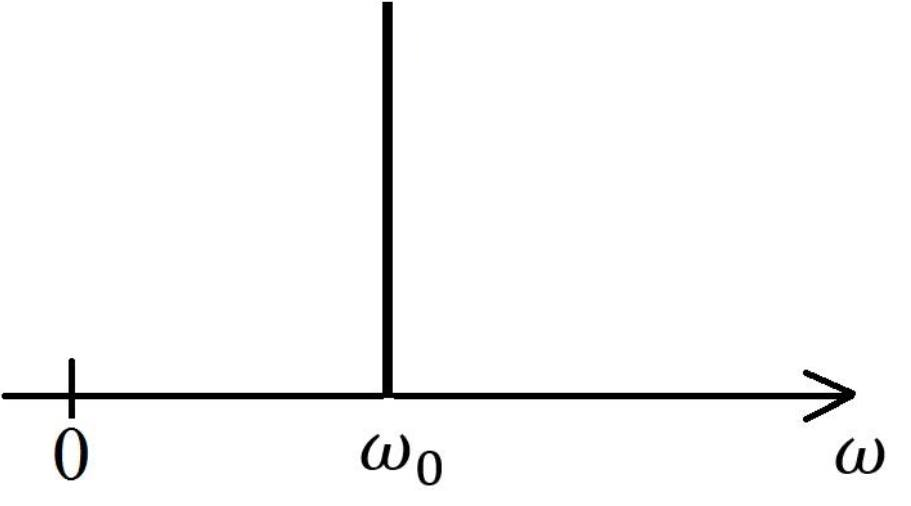
\includegraphics[width=0.8\textwidth]{USPSC-img/sharp_line.png}
		\vspace{5pt}
		\legend{Absorption or emission spectrum without line-broadening mechanisms so that we can assume the line shape $ g(\omega) = \delta(\omega - \omega_0) $.}
		\label{fig:shap-spectral-line}
	\end{subfigure}
	\hfill
	\begin{subfigure}[t]{0.45\textwidth}
		\centering
		\subcaption{Broadened spectral line}
		\vspace{8pt}
		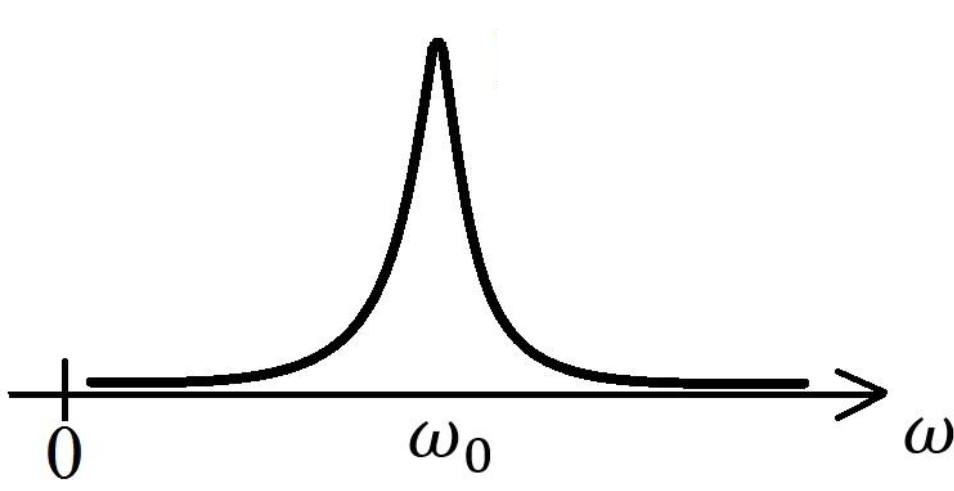
\includegraphics[width=0.8\textwidth]{USPSC-img/broadened_line.png}
		\vspace{5pt}
		\legend{Absorption or emission spectrum taking line-broadening mechanisms into account.}
		\label{fig:broadened-spectral-line}
	\end{subfigure}

	\legend{Source: \cite{valverde2016mecanismos}}
	\vspace{-20pt}
	\label{fig:spectral-broadening}
\end{figure}

We can take these mechanisms into account by introducing the normalized function $ g $ called \textbf{line shape function}. This function can be understood as the probability of absorbing or emitting a photon with frequency between $ \omega $ and $ \omega + d\omega $. A common $ g $ function in atomic spectroscopy is the \textit{Lorentzian}\footnote{Some authors define this distribution as a function of the frequency $ \nu $ instead of the angular frequency $ \omega = 2\pi\nu $.} (Cauchy distribution) given by
\begin{equation}
	g(\omega) = \frac{\Gamma'}{2\pi} \frac{1}{(\omega - \omega_0)^2 + (\Gamma' / 2)^2}\ \ \textrm{or}\ \ g(\Delta) = \frac{\Gamma'}{2\pi} \frac{1}{\Delta^2 + (\Gamma' / 2)^2},
\end{equation}
where $ \Delta = \omega - \omega_0 $ is the \textbf{detuning} and $ \Gamma' $ is the full width at half maximum (FWHM) also known as \textbf{spectral linewidth}. The main spectral linewidth is $ \Gamma' = A $, which is related to the energy-time uncertainty principle. Thus,
\begin{equation}
	g(\omega) = \frac{A}{2\pi} \frac{1}{(\omega - \omega_0)^2 + (A / 2)^2}\ \ \textrm{or}\ \ g(\Delta) = \frac{A}{2\pi} \frac{1}{\Delta^2 + (A / 2)^2}.
	\label{eq:line-shape-simplest-case}
\end{equation}

The probability distribution of finding an atom in the excited state taking the line shape function into account is given by
\begin{equation}
	\rho(t) = (1 - 2P) B \int_{0}^{\infty} u(\omega) g(\omega) d\omega - A P.
	\label{eq:distribution-upper-level-line-shape}
\end{equation}
For a broadband electromagnetic field, which means $ u(\omega) $ much broader than $ g(\omega) $, the equations (\ref{eq:distribution-upper-level-line-shape}) and (\ref{eq:distribution-upper-level}) are equivalent because
\begin{equation}
	\int_{0}^{\infty} u(\omega) g(\omega) d\omega \simeq u(\omega_0) \int_{0}^{\infty} g(\omega) d\omega = u(\omega_0).
	\label{eq:broadband-light-relation}
\end{equation}

%
%-----------------------------------
\subsection{Monochromatic light field}
%-----------------------------------
%

Let us consider a monochromatic electromagnetic field with frequency $ \omega $ interacting with an atom initially in the ground state. In the case, the spectral intensity $ I(\omega) $ and the spectral density energy $ u(\omega) $ of the light field is $ I(\omega') = c u(\omega') = I_0 \delta(\omega' - \omega) $, where $ I_0 $ is the total intensity and $ \delta(x) $ is the Dirac delta. Thus,
\begin{equation}
	\int_{0}^{\infty} u(\omega') g(\omega') d\omega' = \frac{I_0}{c} \int_{0}^{\infty} g(\omega') \delta(\omega' - \omega) d\omega' = \frac{I_0}{c} g(\omega).
	\label{eq:line-broadening-monochromatic-radiation}
\end{equation}
From equation (\ref{eq:distribution-upper-level-line-shape}) and (\ref{eq:line-broadening-monochromatic-radiation}), we obtain
\begin{equation}
	\rho(t) = (1 - 2P) \frac{\alpha(\omega)}{2} - A P,
	\label{eq:distribution-excited-state-monochromatic-light}
\end{equation}
where $ \alpha(\omega) = 2B(I_0 / c)g(\omega) $ is the \textbf{pumping rate}. The stationary solution of (\ref{eq:distribution-excited-state-monochromatic-light}) is given by
\begin{equation}
	P(t) = \frac{1 / 2}{1 + A / \alpha(\omega)} = \frac{1}{2} \frac{s(\omega)}{1 + s(\omega)},
	\label{eq:probability-excited-state-monochromatic-light}
\end{equation}
where $ s(\omega) = \alpha(\omega) / A $ is the \textbf{saturation parameter}, which defines the balance between pumping and relaxation. From equation (\ref{eq:relation-A-B}), we have
\begin{equation}
	s(\omega) = \frac{2\pi^2 c^2}{\hbar \omega_0^3} I_0 g(\omega) = \frac{2\lambda_0^3}{h c} I_0 g(\omega) = \frac{I_0}{I_s} \frac{g(\omega)}{g(\omega_0)},\ \ \textrm{where}\ \ I_s \equiv \frac{\hbar \omega_0^3}{2\pi^2 c^2 g(\omega_0)} .
	\label{eq:saturation-parameter-ERE}
\end{equation}
The intensity $ I_s $ is called \textbf{saturation intensity}. When $ s(\omega) \gg 1 $, stimulated processes are more significant than spontaneous emission, implying the saturation $ P \longrightarrow 1/2 $. When $ s(\omega) \ll 1 $, relaxation processes are predominant. In this case, the atom will certainly decay to the ground state, $ P \longrightarrow 0 $.

%
%-----------------------------------
\subsection{Absorption cross section}
\label{sec:absorption-cross-section}
%-----------------------------------
%

\begin{wrapfigure}{l}{0.45\textwidth}
	\centering
	\caption{Absorption Cross Section}
	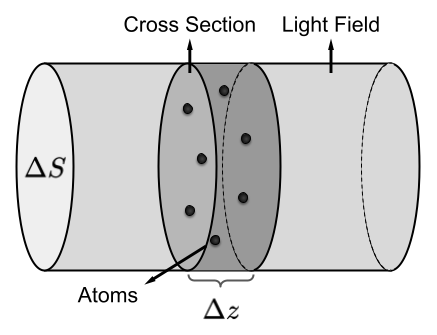
\includegraphics[width=0.43\textwidth]{USPSC-img/cross_section_scheme.png}
	\legend{Dilute atomic gas interacting with a electromagnetic radiation in a slab of thickness $ \Delta z $ and volume $ \Delta S \Delta z $. \\ Source: Author}
	\vspace{-15pt}
	\label{fig:absorption-cross-section}
\end{wrapfigure}

In atomic spectroscopic, it is common to analyze the attenuated or amplified light beam which passes through an atomic medium \cite{reinaudi2007strong, smith2011absorption, shu2004absorption}. Let us consider an electromagnetic beam with total spectral intensity $ I(\omega, z) $ propagating in the z-direction. This radiation passes through an atomic ensemble with $ n_1 $ atoms per volume in the ground state and $ n_2 $ atoms per volume in the excited state (figure \ref{fig:absorption-cross-section}), being attenuated or amplified in each slab of thickness $ \Delta z $ due to stimulated absorption. Its spectral intensity will be reduced by a fraction of $ n_1 \sigma(\omega) \Delta z $, where $ \sigma(\omega) $, known as \textbf{absorption cross-section}\footnote{The absorption cross-section is expressed in units of area}, is related to the probability that an atom will absorb an photon with angular frequency between $ \omega $ and $ \omega + d\omega $ from the light field on the section where this light passes on. Therefore, the lost spectral intensity is given $ \Delta I / I = - N \sigma \Delta z $ and then
\begin{equation}
	\frac{dI}{dz}(\omega, z) = - n_1 \sigma(\omega) I(\omega, z).
	\label{eq:lost-spectral-intensity}
\end{equation}
Besides the light attenuation due to stimulated absorption, there are also gain due to stimulated emission. Spontaneous emission does not contribute to the gain since the emitted light is isotropic. In this case, the light field will be amplified in each slab, increasing its intensity by a fraction of $ n_2 \sigma(\omega) \Delta z $. Here, the quantity $ \sigma $ gives the probability of emitting light stimulately. The absorption cross-section and the emission cross-section are the same since the absorption rate equals the emission rate ($ B_{12} = B_{21} $ when $ g_1 = g_2 $). Therefore, the light gain is given by
\begin{equation}
	\frac{dI}{dz}(\omega, z) = n_2 \sigma(\omega) I(\omega, z).
	\label{eq:spectral-density-power}
\end{equation}
From equations (\ref{eq:lost-spectral-intensity}) and (\ref{eq:spectral-density-power}), we obtain
\begin{equation}
	\frac{dI}{dz}(\omega, z) = - (n_1 - n_2) \sigma(\omega) I(\omega, z)
	\label{eq:net-spectral-density-power}
\end{equation}
where $ (dI / dz) \Delta S \Delta z $ is equivalent to the net spectral power (power per unit of frequency) gained or lost by the radiation in a slab of thickness $ \Delta z $ due to stimulated processes\footnote{Spontaneous emitted light does not come back to the radiation field, since it is isotropic.}. It is convenient to define a \textbf{net absorption cross-section} as 
\begin{equation}
	\sigma_{abs}(\omega) = \frac{n_1 - n_2}{n} \sigma(\omega) = (1 - 2P)\sigma(\omega),
	\label{eq:net-absorption-cross-section}
\end{equation}
where $ n = n_1 + n_2 $ is the total density number and $ P $ is the probability of finding an atom in the excited state. This cross-section is associated with the probability of an atom attenuating or amplifying an incident light due to stimulated processes. Solving the differential equation (\ref{eq:net-spectral-density-power}), we obtain
\begin{equation}
	I(\omega, z) = e^{-n\sigma_{abs}(\omega)t}I(\omega, 0),
	\label{eq:Beer-Lambert-law}
\end{equation}
In the regime of weak excitation such that $ n_2 \ll n_1 $, the total number density is approximately the number density of the atoms in the ground state $ n \simeq n_1 $ and then $ \sigma_{abs}(\omega) \simeq \sigma(\omega) $.

Let us assume a \textit{monochromatic} radiation whose frequency is $ \omega $ such that $  I(\omega', z) = I_0(z) \delta(\omega' - \omega) $ and $ u(\omega', z) = I(\omega', z) / c $. In this case, integrating equation (\ref{eq:net-spectral-density-power}) over all frequencies, we obtain the total power per unit of volume gained or lost by the radiation
\begin{equation}
	\frac{d I_0}{dz}(z) = -n\sigma_{abs}(\omega)I_0(z)\ \ \Rightarrow\ \ I_0(z) = I_0(0) e^{- n\sigma_{abs}(\omega)z}.
	\label{eq:Beer-Lambert-law-total-power}
\end{equation}
In the steady state, $ (dI_0/dz) $ equals the total power per unit of volume lost by spontaneous emission. Then, from equation (\ref{eq:Beer-Lambert-law-total-power}), we have
\begin{gather}
	n\sigma_{abs}(\omega) I_0 = A n_2 \hbar \int_0^{\infty} \omega g(\omega)d\omega.
	\label{eq:cross-section-expression}
\end{gather}
Since $ \omega_0 $ is much greater than the FWHM of $ g(\omega) $\footnote{The line shape function must be normalized over $ 0 $ to $ \infty $, which demands that the peak frequency $ \omega_0 $ of $ g(\omega) $ must be much greater than its FWHM.}, thus
\begin{equation}
	\int_0^{\infty} \omega g(\omega)d\omega \simeq \omega_0.
\end{equation}
Then, from equation (\ref{eq:cross-section-expression}), we have
\begin{equation}
	n \sigma_{abs}(\omega) I_0 = A n_2 \hbar \omega_0\ \Rightarrow\ \sigma_{abs}(\omega) = \frac{\hbar \omega_0}{I_0} A P,
	\label{eq:net-absorption-cross-section}
\end{equation}
where $ P = n_2 / n $. Therefore, in the steady state, the \textit{net absorption cross-section} can be understood as an area on which the photon flux of the incident beam passes through times the rate $ \Gamma P $ at which an atom scatters photons by spontaneous emission, i.e. the decay rate $ \Gamma $ times the probability of finding an atom in the excited state. From equations (\ref{eq:probability-excited-state-monochromatic-light}), (\ref{eq:saturation-parameter-ERE}), and (\ref{eq:net-absorption-cross-section}), we obtain
\begin{gather}
	\sigma(\omega) = \frac{\hbar \omega_0}{I_0} \frac{A}{2} s(\omega) = \overbrace{\frac{\hbar \omega_0}{I_s} \frac{A}{2}}^{\sigma_0} \frac{g(\omega)}{g(\omega_0)} = \sigma_0 \frac{g(\omega)}{g(\omega_0)}\ \ \textrm{and}
	\label{eq:absorption-cross-section-2}
	\\
	\sigma_{abs}(\omega) = \frac{\hbar \omega_0}{I_0} \frac{A}{2} \frac{s(\omega)}{1 + s(\omega)} = \sigma(\omega) \frac{1}{1 + s(\omega)},
	\label{eq:net-absorption-cross-section-2}
\end{gather}
where $ \sigma_0 \equiv \sigma(\omega_0) $ is the \textit{resonant absorption cross-section} which only depends on the properties of the atom ($ I_s$, $ \omega_0 $, and $ A $).



